\documentclass{scrartcl}
\usepackage[headsepline]{scrlayer-scrpage}
\pagestyle{scrheadings}
\usepackage[a4paper, left=3cm, right=3cm, top=3cm]{geometry}
\usepackage[english]{babel}
\usepackage{amsmath,amssymb}
\usepackage{graphicx}
\usepackage{float}
\usepackage{tikz}
\usepackage{caption}
\usepackage{subcaption}
\usepackage{cleveref}

\begin{document}
	
	\title{Machine Learning}
	\subtitle{Exercise 1}
	\author{Jan Kruska | Sagar G. Kalburgi | Kashyap M. Mahesh | Pawan Chand}
	\date{\today}
	%\publishers{Platz für Betreuer o.\,ä.}% optional
	
	\maketitle
	
	\section*{Question 2}
	\subsection*{a)}
	$p(apple) = p(r\cap apple) + p(g\cap apple) + p(b\cap apple)$ \\
	$p(apple) = p(r) * p(apple|r) + p(g) * p(apple|g) + p(b) * p(apple|b)$ \\
	$p(apple) = 0.2 * \frac{3}{10} + 0.6 * \frac{3}{10} + 0.2 * \frac{1}{2} = 0.34 $
	
	\subsection*{b)}
	$p(g|orange) = \frac{p(orange|g)p(g)}{p(orange)}$ \\
	$p(orange) = p(r) * p(orange|r) + p(g) * p(orange|g) + p(b) * p(orange|b)$ \\
	$p(g|orange) = \frac{p(orange|g)p(g)}{p(r) * p(orange|r) + p(g) * p(orange|g) + p(b) * p(orange|b)}$ \\
	$p(g|orange) = \frac{0.3*0.6}{0.2*0.4 + 0.6*0.3 + 0.2*0.5} = 0.5$ \\
	
	
	\section*{Question 6}
	\subsection*{a-e}
	See attached python code.
	
	The provided EStep function is parallelized, but likely to only run on unix-systems. For testing on non-unix systems delete the underscore in front of the function-name of the serialized version and put one in front of the parallelized version.
	(Efficiency of the parallelization isn't really great though. I reach a speedup of the Estep function of about $3.5$ with 12 Threads on my machine)
	
	\subsection*{f)}
	\begin{figure}[h]
		\centering
		\begin{subfigure}[b]{0.3\textwidth}
			\centering
			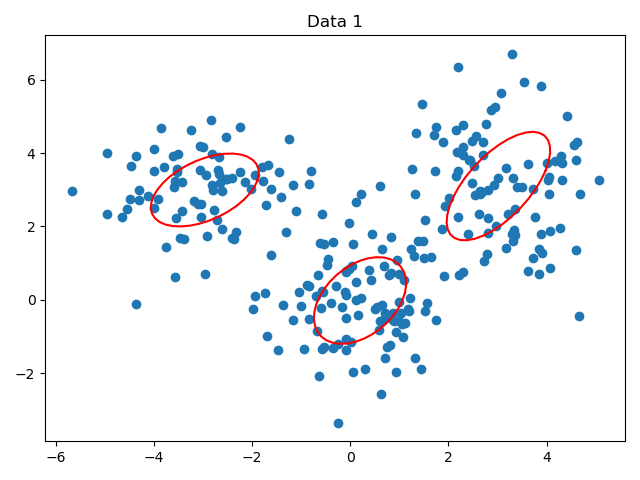
\includegraphics[width=\textwidth]{images/data1}
			\caption{GMM on Data 1}
		\end{subfigure}
		\hfill
		\begin{subfigure}[b]{0.3\textwidth}
			\centering
			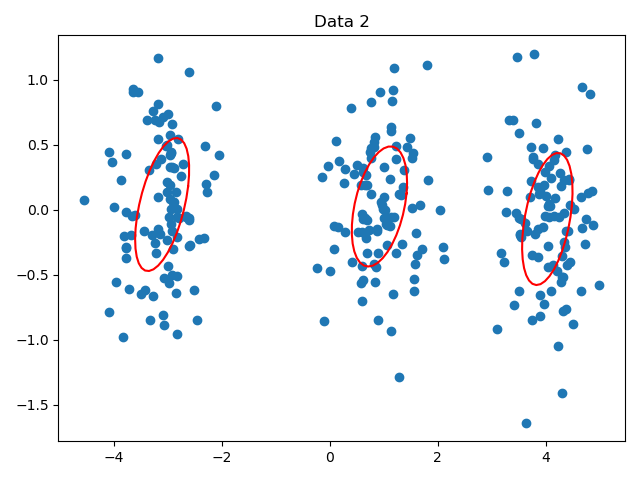
\includegraphics[width=\textwidth]{images/data2}
			\caption{GMM on Data 2}
		\end{subfigure}
		\hfill
		\begin{subfigure}[b]{0.3\textwidth}
			\centering
			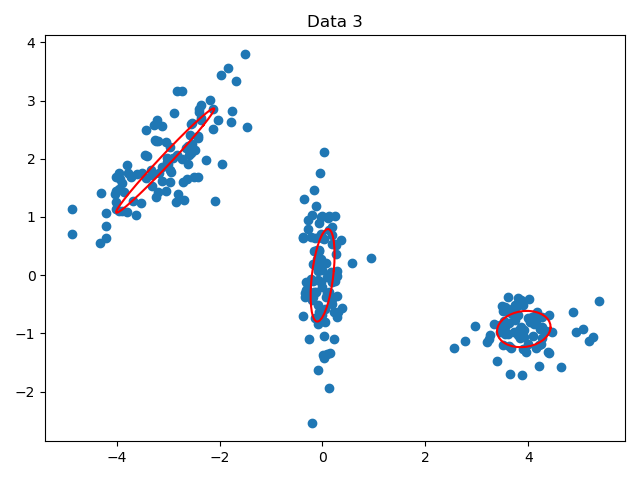
\includegraphics[width=\textwidth]{images/data3}
			\caption{GMM on Data 3}
		\end{subfigure}
		\caption{GMM-models on the three provided datasets}
		\label{fig:three graphs}
	\end{figure}

\begin{figure}
	\centering
	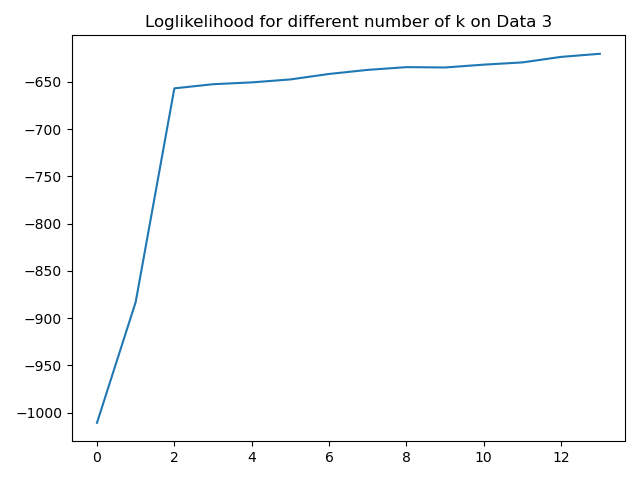
\includegraphics[width=.5\textwidth]{images/data3loglikelihood}
	\caption{Loglikelihood on third dataset over different numbers of K}
\end{figure}
\subsection*{g)}
\begin{figure}[h]
	\centering
	\begin{subfigure}[b]{0.45\textwidth}
		\centering
		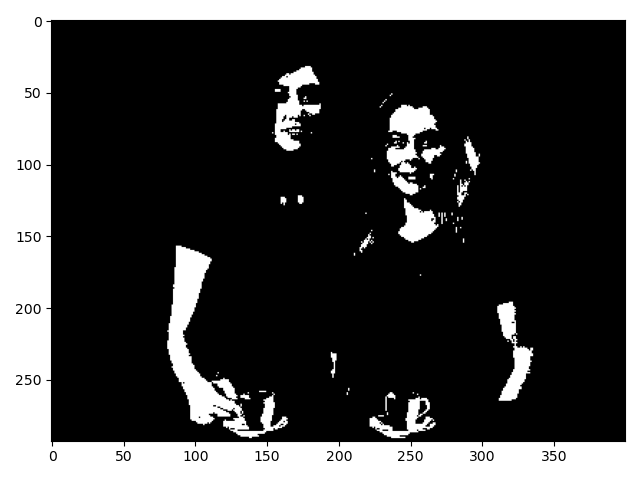
\includegraphics[width=\textwidth]{images/skinTheta0.7}
		\caption{$\theta=0.7$}
	\end{subfigure}
	\hfill
	\begin{subfigure}[b]{0.45\textwidth}
		\centering
		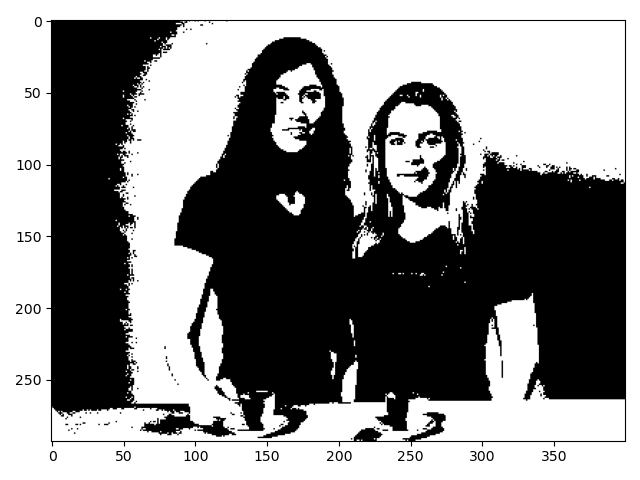
\includegraphics[width=\textwidth]{images/skinTheta0.6}
		\caption{$\theta=0.6$}
	\end{subfigure}
	\hfill
	\quad
	\begin{subfigure}[b]{0.45\textwidth}
		\centering
		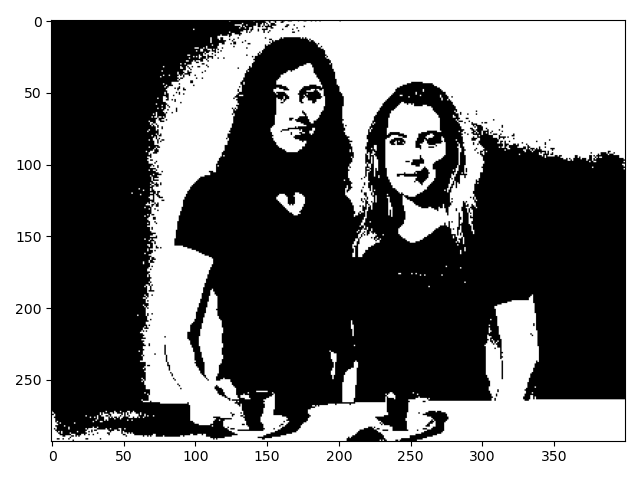
\includegraphics[width=\textwidth]{images/skinTheta0.65}
		\caption{$\theta=0.65$}
	\end{subfigure}
\hfill
\begin{subfigure}[b]{0.45\textwidth}
	\centering
	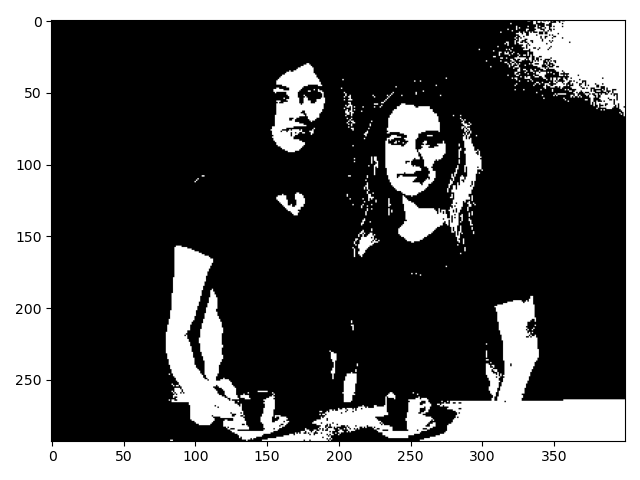
\includegraphics[width=\textwidth]{images/skinTheta0.68}
	\caption{$\theta=0.68$}
\end{subfigure}
	\caption{Skin detection}
	\label{fig:skin}
\end{figure}
The main problem with skin detection is the fact, that the light parts of the background are quite similar in color to skin.
Due to that fact 
With $\theta=0.7$ the current model reaches a precision of $0.98$ on the training data \footnote{I know that a train-test-validation-split would provide in more meaningful results, but I didn't have time to split the data (Also I only realized now that one could/should probably use the picture for validation)}, so at that point there are very few false positives.
However the recall is $~0.54$, so a large amount of skin pixels in the training dataset are already missed. The $F_1=0.69$  isn't that remarkable, but it shows that the solution is somewhat feasible

Lowering $\theta$ to $0.6$ drastically lowers precision to $0.66$, while increasing recall to $0.78$, resulting in an $F_1=0.72$

Moving inside this band to $\theta=0.65$ did not lead to a big improvement (precision $0.71$, recall $0.76$, $F_1=0.74$) and large parts of the background are still misclassified, as can be seen in the \cref{fig:skin}

The best classification performance that we reached was with a $\theta=0.68$, which increased precision to $0.87$ recall to $0.72$ with an $F_1=0.79$.
The result can be seen in \cref{fig:skin} d), and provides a decent segmentation, though parts of the well-lit background and table are classified as skin, whereas badly-lit bodyparts are already missed.

Interestingly raising $K$ did not seem to help much. Any values for $K>4$ did not really increase any quality measure.
The models already converged with $5$ Iterations, but a combination of raising $K$ and the number of iterations could provide better results.

Generally a more rigorous approach towards the hyperparamters would be advisable

Also utilizing neighbourhood relations, which are natural in images, i.e. that skin pixels are most likely next to other skin pixels, could greatly improve classification performance.


\end{document}